\documentclass[12pt]{article}

\usepackage{sbc-template}

\usepackage{graphicx,url}
\usepackage{placeins}
\usepackage{subfigure}

\usepackage{multirow}
\usepackage[brazil]{babel}    
\usepackage[utf8]{inputenc}
 
\sloppy

\title{Comparação do número de acessos à memória e TLB \textit{misses} com
páginas de 4KB ou 4MB}

\author{Gustavo Ciotto Pinton\inst{1} }


\address{Instituto de Computação -- Universidade Estadual de Campinas
(UNICAMP)\\
  Av. Albert Einstein, 1251, Cidade Universitária, Campinas/SP \\
  Brasil, CEP 13083-852, Fone: [19] 3521-5838
  \email{ra117136@unicamp.br}
}

\begin{document}  

\maketitle

\begin{abstract}
This report describes the number of TLB misses for data and instruction, in
addition to memory and page table accesses executed by the \texttt{SPEC CPU2006}
benchmarks with the largest memory footprints. Such measures were achieved
thanks to the implementation of a new pintool, capable of modelling data and
instruction TLB caches with 4KB and 4MB memory pages. In this report, we have
considered L1, L2 and L3 caches with different size in order to compare the
total memory table  accesses with total memory accesses. Besides, in order to
get test results faster, we used Intel's Program Record/Replay Toolkit (pinplay)
with SPEC CPU2006 pinballs downloaded from the Internet corresponding to the
\texttt{ref} input set. Finally, we wrote a toy benchmark to test memory access
and allocation exclusively.
\end{abstract}
     
\begin{resumo} 
Este relatório apresenta o número de acessos à memória, à tabela de páginas e
TLB \textit{misses} para os \textit{benchmarks} do \texttt{SPEC
CPU2006} com maiores \textit{memory footprints}. Tais medidas foram
realizadas através da implementação de uma nova pintool, capaz de reproduzir o
modelo de TLB de instruções e dados com páginas de 4KB e 4MB. Neste relatório,
foram considerados os níveis L1, L2 e L3 de cache a fim de compararmos o efeito
dos acessos à tabela de páginas em relação aos acessos totais à memória.
Além disso, a fim de agilizar os testes, fez-se uso da ferramenta pinplay, também desenvolvida
pela Intel, para a execução da respectiva pintool. Os pinballs foram retirados
da Internet e correspondem ao testes cujas entradas correspondem ao conjunto
\texttt{ref}. Por fim, implementou-se um benchmark adicional com intuito de
testar exclusivamente a alocação e acesso da memória.
\end{resumo}

\section{Introdução}

O espaço de endereço \textit{físico} é definido como o intervalo de endereços
que podem ser utilizados para indexar efetivamente a memória física de um
dispositivo e que podem ser gerados pelo processador no seu barramento. O espaço
de endereço \textit{virtual}, por sua vez,  é o intervalo de endereços que uma
aplicação pode utilizar. Cabe ao sistema operacional gerenciar o mapeamento
entre estes dois \textit{tipos} de memória. A virtualização de um programa
oferece duas vantagens principais. A primeira corresponde ao fato de que
programas não precisam ser alterados quando executados em máquinas com
diferentes tamanhos de memória física. Em segundo, a virtualização garante a
proteção do espaço de memória de cada aplicação, à medida que isola seus espaços
de memória virtual através de alguns \textit{bits} adicionais. 

O espaço de endereços, tanto o virtual como o física, é dividido em
\textit{páginas}, que neste relatório, terão tamanho de 4KB ou 4MB. Uma página
pode ser armazenada tanto na memória principal quanto em disco, caso a primeira
esteja já totalmente ocupada. O sistema operacional realiza toda a gerência da
memória física, cabendo a ele alocar ou desalocar (inclusive, em que endereço)
páginas e atribuir endereços físicos aos virtuais utilizados pelas diversas
aplicações. Esse mapeamento é realizado através de uma estrutura chamada de
\textit{tabela de páginas}, que é mantida em um endereço especial da memória
principal.

É importante lembrar que duas ou mais páginas virtuais podem ser mapeadas para
uma mesma página física da memória. Essa técnica, chamada de \textit{virtual
addressing}, é utilizada em aplicações que compartilham memória entre si, como,
por exemplo, em bibliotecas tais como a \textit{glibc} e requer mecanismos
especiais de atualização de \textit{caches} ou \textit{buffers}, uma vez que
mudanças realizadas em uma das aplicações devem ser refletidas nos demais.

Uma possível implementação da tabela de páginas, visando a economia de memória,
é através de um sistema multi-níveis ou hierárquico. Neste caso, o endereço que 
deve ser traduzido é dividido em \(N+1\) seções, em que \(N\) representa o
número de níveis escolhido. Cada uma das seções possui o índice da tabela
ocupado pelo endereço naquele respectivo nível, sendo que uma tabela é composta
por ponteiros para tabelas do próximo nível.
% Por exemplo, se em uma máquina de
% 32 \textit{bits}, uma página tivesse 4KB e cada entrada ocupasse 4
% \textit{bytes}, e se houvesse apenas um nível, a tabela completa ocuparia \(4 *
% 2 ^{10} * 4 = 2 ^ {14}\) \textit{bytes} na memória. Desta maneira, para acessar apenas um
% dado, seriam necessários \(2 ^ {14}\) \textit{bytes}. Por outro lado, se
% 2 níveis fossem utilizados e se 10 \textit{bits} fossem usados para indexar cada
% um dos dois níveis, teríamos \(4*2 ^{10}\) = 4KB para o primeiro nível e
% outros 4KB para o segundo. Assim, neste caso, precissaríamos de apenas 8KB, representando
% uma economia de \(\frac{2 ^ {14}}{8 * 2 ^{10}} = 2\) vezes. Para a implementação
% da \textit{pintool}, assumiu-se que essa hierarquia possuia 3 níveis.

Durante a execução de um programa, muitas operações de leitura (de instruções
e dados) e escrita na memória são requisitadas. Para cada uma destas operações,
o mapeamento teria que ser obtido e diversos outros acessos
adicionais à memória seriam realizados (para um tabela de páginas com 3
níveis, por exemplo, seriam necessários 3 outros acessos), resultando, assim,
na degradação da sua performance. Para evitar este cenário, um cache da tabela
de página é adicionado aos processadores e é chamado de TLB, do inglês
\textit{Translation Lookaside Buffer}. Tal cache recebe como entrada o número da
página virtual e devolve, em caso de sucesso, o respectivo número da página
física e algumas informações adicionais, como permissão de escrita e processo
que a detém. Para a nossa aplicação, modelamos dois caches TLB completamente
associtativos, um para as instruções e outro para os dados, com 512 entradas
cada. Além disso, modelamos três níveis de cache, sendo eles L1, L2 e L3, de
acordo com as informações contidas em \cite{intel} para o processor i3.
O primeiro nível contém dois caches dedicados para instruções e dados,
separadamente, com 32KB cada e 8-way associative. O segundo nível, L2, é
unificado para instruções e dados, possuindo 256KB e 8-way associative. Por fim,
o cache L3, possui 4MB, sendo 16-way associative.

Neste relatório, serão avaliados dois modelos com páginas de 4KB e 4MB. Para
tal, uma nova \textit{pin tool} foi escrita com base nas implementações de cache
disponíveis no próprio diretório do \textit{pin}. Os testes foram realizados nos
\textit{benchmarks} com maior \textit{memory footprint} através da ferramenta
\textit{pinplay}, cujos \textit{pinballs} foram retirados da Internet. Foram
escolhidos os \textit{pinballs} com 100M de instruções executadas como
\textit{warmup}, regiões de 30M instruções e máximo do parâmetro K do
algoritmo de clusterização igual a 10 \cite{pinballs}. 

\section {Implementação da \textit{pin tool}}

O arquivo \texttt{pin\_cache.H}, disponível no diretório de instalação do
\textit{pin}, fornece algumas classes que modelam o funcionamento de um cache.
As classes \texttt{ROUND\_ROBIN} e \texttt{DIRECT\_MAPPED} modelam  e
implementam duas politícas de substituição. A primeira consiste na implementação
de uma lista circular através de um vetor, em que elementos são inseridos no fim
da lista e retirados do começo. Neste caso, diferentemente da politíca LRU, não há
quaisquer registros sobre a última utilização de uma entrada: tende-se a
acreditar que elementos mais próximos do início da fila foram usados há mais
tempo e, por isso, a probabilidade de serem novamente acessados é menor. A
política \texttt{DIRECT\_MAPPED}, por sua vez, é trivial, já que representa um
conjunto com apenas um elemento (associatividade igual a 1). A estrutura do
cache é representada pela classe \texttt{CACHE\_BASE}, que fornece uma série de
métodos permitindo o controle das estatísticas dos acessos ao cache. Tal classe
é extendida por \texttt{CACHE}, que acrescenta métodos de modificação do conteúdo
armazenado. Os dois principais métodos são \texttt{AccessSingleLine} e
\texttt{Access}, responsáveis por acessar uma ou múltiplas linhas do cache,
respectivamente, retornando \textit{true} em caso de \textit{hit} e
\textit{false}, caso contrário. Estes dois métodos também se encarregam da
substituição, em caso de \textit{miss}, de uma das entradas pelo novo elemento.

A \textit{pintool} instancia 7 caches distintos: 2 para páginas de 4KB, 2 para
páginas de 4MB e três para os níveis L1, L2 e L3. Não há a necessidade de
criarmos instâncias distintas para os 3 últimos, visto que os endereços
procurados são os mesmos, tanto no caso de páginas de 4KB como no de 4MB. Cada
um dos pares de TLB é constituído por um TLB para os dados e outro para as
instruções. Todos eles são completamente associativos, utilizam a política de
substituição \textit{round robin} e possuem 512 entradas. O
primeiro nível L1 contém dois caches dedicados para instruções e dados,
separadamente, com 64KB cada e 32-way associative. O segundo nível, L2, é
unificado para instruções e dados, possuindo 256KB e 8-way associative. Por fim,
o cache L3, possui 4MB, sendo 16-way associative. As rotinas de instrumentação são
colocadas a cada \textit{trace} através da chamada da função
\texttt{TRACE\_AddInstrumentFunction()} e as de análise, antes de cada bloco
funcional (também chamado de \textit{basic block}) ou instrução, dependendo da
sua natureza. Dentro da função de instrumentação, itera-se sobre todos os
\textit{basic blocks} a partir das funções \texttt{TRACE\_BblHead()} e
\texttt{BBL\_Next()} e, para cada um deles, uma função de análise é registrada,
cujo propósito é verificar o número de acessos à memória referente à fase de
\textbf{instruction fetch}. Nesta etapa, o processador busca na memória as
instruções a serem executadas. Esta função de análise recebe, além do endereço
inicial do bloco, o seu tamanho e realiza a chamada dos métodos
\texttt{Access()} de cada um dos TLBs de instrução. Ainda na função de
instrumentação, itera-se também sobre as instruções de cada \textit{basic block}
em busca de operações de \textit{load} ou \textit{store}. Caso uma delas seja
encontrada, então uma função de análise é registrada, recebendo como parâmetro o
endereço de escrita ou leitura. A finalidade desta última é chamar um dos dois
métodos de acesso (\texttt{AccessSingleLine()} ou \texttt{Access()}) dos TLBs de
dados, dependendo do tamanho dos operadores.

Diferentemente do projeto 1, a degradação no desempenho dos
\textit{benchmarks} neste caso é proibitivo, exigindo um tempo muito elevado
para as execuções do tipo \texttt{ref}. Uma ferramenta proposta para minimizar
este problema é o \textit{Program Record/Replay Toolkit}, que permite
salvar ou carregar estados inteiros de uma execução, chamados também de
\textit{pinballs}. Aliado a este \textit{toolkit},
pesquisadores da faculdade da California desenvolveram uma ferramenta capaz de
detectar as regiões mais representativas, chamadas de \textit{SimPoints}, a
partir de análise de fases em execuções de grandes programas. Eles mostraram
que a execução de apenas estas regiões é capaz de revelar com uma precisão muito
grande o desempenho real do programa. Ainda com base nestes conceitos, os
pesquisadores da Intel extenderam a ideia para criar \textit{PinPoints}, isto é,
regiões representativas de análise compatíveis com o \texttt{pin}. Enfim,
pesquisadores da Universidade de Ghent disponibilizaram os \textit{pinballs}
relativos às execuções dos \textit{benchmarks} do \texttt{SPEC CPU2006} para as
entradas do conjunto \texttt{ref}. A seção \textit{Resultados}, a seguir,
representa, portanto, os resultados encontrados executando-se o \textit{Program
Record/Replay Toolkit} com tais \textit{pinballs}.

\section {Implementação de um \textit{toy benchmark}}

A fim de testarmos exclusivamente o desempenho da memória, um \textit{benchmark}
foi escrito.  De maneira geral, este \textit{benchmark} aloca vetores de
inteiros e pontos flutuantes e realiza acessos aleatórios a eles. Espera-se que
os acessos aleatórios produzam muitas \textit{cache misses}, forçando, assim,
mais acessos à memória. 

A fim de aumentar a quantidade de memória utilizada, o programa aloca dois
vetores, um de ponteiros para inteiro (\texttt{int*})
e outro de ponteiros para ponto flutuante de precisão dupla (\texttt{double*}).
Para cada um dos ponteiros presentes nestes vetores, são alocados novos vetores. 
Neste relatório, chamamos de primeiro nível a alocação de vetores dos tipos
\texttt{int*} ou \texttt{double*} e de segundo nível a alocação de vetores dos
tipos primitivos \texttt{int} ou \texttt{double}. É necessário observar que a
alocação sempre ocupa páginas inteiras de memória, isto é, por exemplo, o vetor
\texttt{int*} de primeiro nível terá \texttt{NUMBER\_OF\_PAGES\_LEVEL\_1} *
\texttt{PAGE\_SIZE} / \texttt{sizeof(int*)}. As constantes abaixo são
definidas, a fim de facilitar o entendimento:

\begin {itemize}
\item  \texttt{PAGE\_SIZE}: tamanho de cada página de memória. Definida como
4KB.
\item  \texttt{NUMBER\_OF\_PAGES\_LEVEL\_1}: número de páginas ocupadas no
primeiro nível para cada vetor. Por padrão, 512.
\item  \texttt{NUMBER\_OF\_PAGES\_LEVEL\_2}: número de páginas ocupadas no
segundo nível para cada vetor. Por padrão, 1.
\item  \texttt{RANDOM\_ACCESSES}: número de acessos aleatórios aos vetores.
Definida inicialmente como 15000.
\end{itemize}

Com o teste deste \textit{benchmark}, espera-se um desempenho muito ruim da
TLB de 4KB nos acessos aleatórios, já que produzirão muitos \textit{TLB misses},
mas, ao contrário, bom com o de 4MB, visto que 1024 páginas de 4KB podem ser
contidas dentro de uma de 4MB. Observa-se que são necessárias apenas duas
páginas de 4MB para conter os dois níveis, sendo assim, poucos \textit{misses}
de dados são esperados. Além disso, considerando que o código não é extenso,
espera-se também que não haja muito \textit{misses} no cache de instruções.

\section {Resultados}

Esta seção visa a análise dos resultados obtidos tanto para os
\textit{benchmarks} selecionados do SPEC, quanto para o \textit{toy benchmark}
criado.

\subsection{Resultados para os \textit{benchmarks} do \texttt{SPEC2006}}

Visamos escolher os 10 \textit{benchmarks} com maiores \textit{footprint} e,
para tal, baseamos-nos em \cite{Henning:07}. Este trabalho apresenta os
atributos \textit{rss}, \textit{vsz} dos \textit{benchmarks}, assim como as suas
estabilidades. O primeiro atributo, \textit{rss}, é uma abreviação para
\textit{resident set size} e representa a memória física alocada, enquanto que a
segundo, \textit{vsz} ou \textit{virtual size}, indica o tamanho total e memória
virtual utilizada. Enfim, um \textit{benchmark} é considerado estável se o
consumo de memória cresce rapidamente aos valores medidos e se mantém neste
nível. % A tabela \ref{table:bench} contém os \textit{benchmarks} selecionados.
Observa-se que a maioria dos \textit{benchmarks} do conjunto inteiro não são
estáveis, contrariamente aos do conjunto de ponto flutuante, e, de maneira
geral, os \textit{benchmarks} deste último consomem mais memória (dos dois
\textit{tipos}, inclusive).

% \begin{table}[h]
%     \centering
% 	\caption{\label{table:bench} \textit{Benchmarks} selecionados. Medidas estão
% 	em MB. Extraído de \cite{Henning:07}.}
% 	\begin{tabular}{| c | c | c | c | c | c | c | c |}
% 		\hline
% 		\multicolumn{4}{|c|}{ \texttt{SPECint2006}} & \multicolumn{4}{|c|}{
% 		\texttt{SPECfp2006}} \\ \hline \textbf{Benchmark} & \textbf{rss} & \textbf{vsz} &
% 		\textbf{Estável?} & \textbf{Benchmark} & \textbf{rss} & \textbf{vsz} &
% 		\textbf{Estável?} \\ \hline
% 		
% 		400.perlbench & 580 & 581 & N & 410.bwaves & 881 & 894  & S \\ \hline
% 		401.bzip2 & 856 & 856 & N &  434.zeusmp & 525 & 1138 & S \\ \hline
% 		403.gcc & 932 & 933 & N & 436.cactusADM  & 879 & 1018 & S \\ \hline
% 		429.mcf & 844 & 845 & S & 459.GemsFDTD & 838 & 850 & S \\ \hline
% 		& & & & 481.wrf & 701 & 718 & N \\ \hline
% 		& & & & 433.milc & 676 & 677 & N \\ \hline
% 		
% 		\hline
% 	\end{tabular}	    
% \end{table}

Os caches L1, L2 e L3 apresentam os mesmos resultados para \textit{misses} e
\textit{hits} considerando os dois tamanhos de páginas. Isso ocorre devido ao
fato de que os endereços procurados são os mesmos nos dois casos e, portanto,
em termos de acessos a tais caches não há alguma diferença. Por outro lado, os
resultados das conversões realizadas pelas TLBs sofrem modificações, visto que,
com páginas de tamanhos distintos, a página física alocada para determinado
dado ou instrução pode mudar. Para páginas maiores, por exemplo, a chance que dados
acessados dentro de intervalos de tempo muito curtos estejam na mesma página é
maior que para páginas de tamanhos pequenos. Por efeitos de simplicidade, a
tabela \ref{tabela:l123s} representa apenas os dados referentes ao último
nível L3, obtidos para as execuções:

\vspace{-12pt}

\begin{table}[h]
    \centering
	\caption{\label{tabela:l123s} \textit{Misses} e \textit{Hits} obtidos no
	nível L3.}
	\begin{tabular}{| c | c | c | c | c | c |}
		\hline
		\multicolumn{3}{|c|}{ \texttt{SPECint2006}} & \multicolumn{3}{|c|}{
		\texttt{SPECfp2006}} \\ \hline \textbf{Benchmark} & \textbf{Hits} &
		\textbf{Misses} & \textbf{Benchmark} & \textbf{Hits} &
		\textbf{Misses} \\ \hline
		
		perlbench & 166215 & 138697 & bwaves & 14242 & 1272419  \\ \hline
		bzip2 & 689006 & 109176 &  zeusmp & 226840 & 824567  \\ \hline
		gcc & 1899809 & 112876 & cactusADM  & 121457 & 562178  \\ \hline
		mcf & 3807099 & 6566234  & GemsFDTD & 378415 & 1296796 \\ \hline
		& & & wrf & 123376 & 813526  \\ \hline
		& & & milc & 26664 & 3242983  \\ \hline
		
		\hline
	\end{tabular}	    
\end{table}

Cada \textit{miss} na tabela acima corresponde a um acesso à memória. As
figuras \ref{fig:int4K} e \ref{fig:data4K} representam o total de
acessos devido a instruções e a dados para páginas de 4KB, respectivamente. As
figuras \ref{fig:int4M} e \ref{fig:data4M}, por sua vez, representam os mesmos
números, só que para páginas de 4MB. Para cada \textit{benchmark}, a
barra na extremidade esquerda representa o total número de acessos, a
do meio, o número de \textit{misses} na TLB e, a da direita, o número
de acessos à tabela de páginas ocassionados por ela. Todos os gráficos
estão em escala logarítimica. Observa-se que:

\begin{itemize}
  \item O número de acessos adicionais causados por \textit{misses} na TLB de
  instruções em páginas de 4KB corresponde a uma fração importante do número de
  acessos total. O mesmo ocorre para acessos ocasionados por leitura e escrita
  de dados.

  \item Para páginas de 4MB, o número de \textit{misses} na TLB de instruções é
  praticamente nulo. Os acessos à memória são gerados exclusivamente por
  \textit{misses} em L3. Esse desempenho já era esperado, já que utiliza-se
  maiores espaços de armazenamento. Por outro lado, páginas deste comprimento
  tendem a provocar uma maior fragmentação da memória, à medida que até
  processos pequenos passariam a ocupar 4MB no mínimo.
%   Se comparado com o caso anterior, este caso apresenta
%   uma grande economia de tempo, porém utiliza uma maior área para a TLB.
%   Dependendo da área e \textit{design} interno do processador, é necessário
%   avaliar corretamente quais benefícios são mais importantes.

  \item Para os dados em páginas de 4MB, apesar do número de acessos à tabela de
  páginas ser muito inferior àquele de 4KB, ele ainda apresenta uma fração
  considerável no total de acessos. Isto indica que, mesmo com páginas de grande
  comprimento, é necessário que o sistema operacional implemente algoritmos
  eficientes de escrita e leitura de entradas na tabela de páginas.
\end{itemize}

\begin{figure}[h]
  \centering
  \subfigure[Acessos à memória devido a instruções. Páginas de 4KB.]{%
    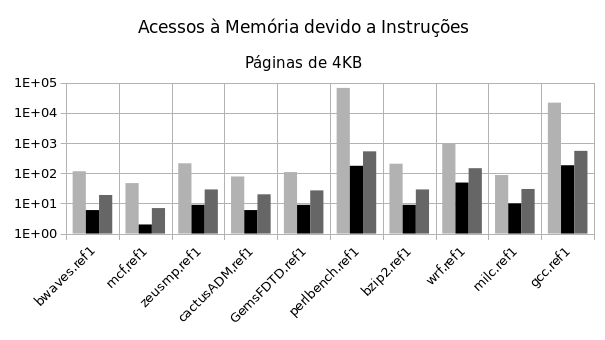
\includegraphics[width=0.49\textwidth]{img/inst_4KBs}%
    \label{fig:int4K}%
  }%
  \hfill
  \subfigure[Acessos à memória devido a dados. Páginas de 4KB.]{%
    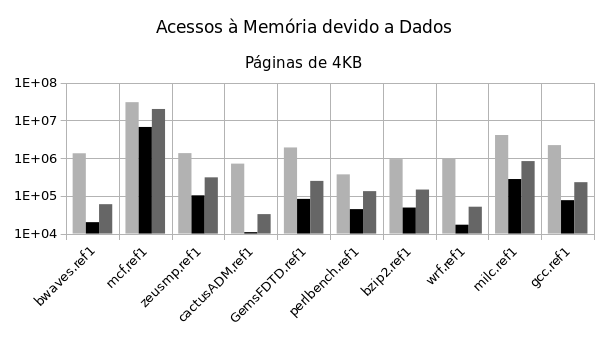
\includegraphics[width=0.49\textwidth]{img/data_4KBs}%
    \label{fig:data4K}%
  }
  \caption{Acessos à memória devido a instruções e dados para páginas de 4KB.}
\end{figure}
  
\begin{figure}[h]
  \subfigure[Acessos à memória devido a instruções. Páginas de 4MB.]{%
    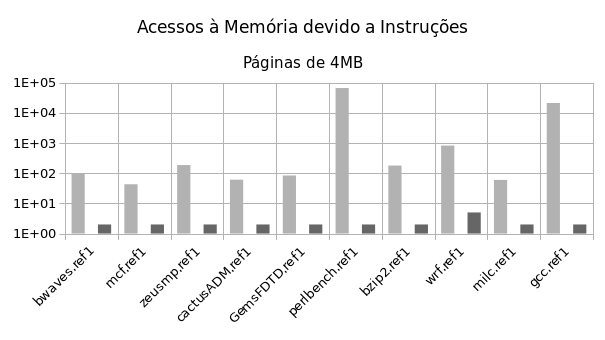
\includegraphics[width=0.49\textwidth]{img/inst_4MBs}%
    \label{fig:int4M}%
  }%
  \hfill
  \subfigure[Acessos à memória devido a dados. Páginas de 4MB.]{%
    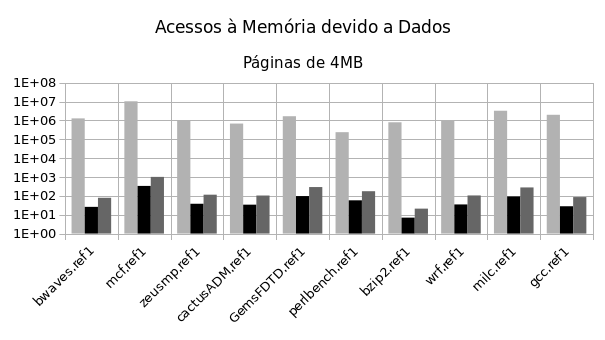
\includegraphics[width=0.49\textwidth]{img/data_4MBs}%
    \label{fig:data4M}%
  }%
  \caption{Acessos à memória devido a instruções e dados para páginas de 4MB.}
  \label{fig:acessos}
\end{figure}


\subsection{Resultados para o \textit{toy benchmark}}

As figuras \ref{fig:toyi} e \ref{fig:toyd} representam o resultado da execução
deste \textit{benchmark}. Verifica-se, conforme esperado, que a quantidade de
\textit{misses} nas TLBs é muito superior para o caso de páginas de 4KB. Para as
instruções, a quantidade de misses para tal caso é praticamente 10 vezes maior
que o caso de páginas de 4MB. Para dados, esta diferença é ainda maior: cerca de
1000 vezes maior. Tais fatos indicam que, para programas adaptados para
determinado tamanho de página, seu desempenho pode ser altamente degradado caso
ele seja executado em outro ambiente. 

\begin{figure}[h]
  \centering
  \subfigure[Acessos à memória devido a instruções.]{%
    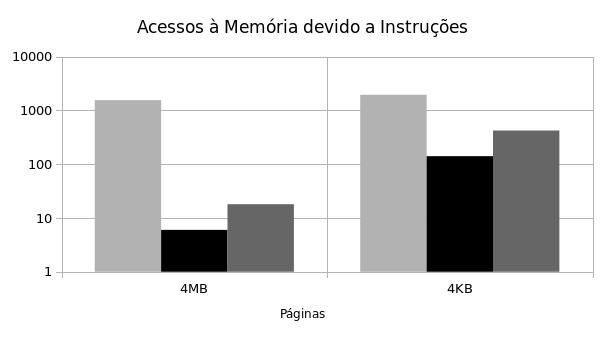
\includegraphics[width=0.49\textwidth]{img/toy_inst}%
    \label{fig:toyi}%
  }%
  \hfill
  \subfigure[Acessos à memória devido a dados.]{%
    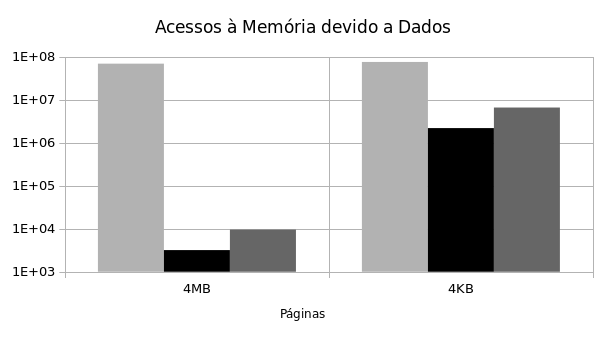
\includegraphics[width=0.49\textwidth]{img/toy_data}%
    \label{fig:toyd}%
  }
  \caption{Acessos à memória devido a instruções e dados para páginas de 4KB e
  4MB.}
\end{figure}

\section {Conclusões}

Neste projeto, foi possível avaliar o impacto nos caches de TLB, L1, L2 e L3 de
páginas de tamanhos distintos. Páginas de 4KB produzem mais \textit{misses} nas
TLBs de dados e instruções, gerando assim mais acessos à memória. Por outro
lado, tais caches são menores, ocupando uma área menor dentro do
processador e produzem menos fragmentação de memória. Páginas de 4MB, por sua
vez, diminuem significamente o número de acessos à tabela de páginas, mas ocupam uma área muito superior e produzem
muita fragmentação de memória à medida que o número de processos aumenta. É
preciso, portanto, avaliar os \textit{tradeoffs} das duas soluções e avaliar
quais benefícios serão priorizados no \textit{design} de um processador.

\bibliographystyle{sbc}
\bibliography{sbc-template}

\end{document}
 